\documentclass{beamer}

\usetheme{Madrid}
\usepackage[backend=biber]{biblatex}
\addbibresource{mybib.bib}
\usepackage{graphicx}
\usepackage{amsmath}
\usepackage{amssymb}
\usepackage{amsthm}

\makeatletter
\newcommand{\vo}{\vec{o}\@ifnextchar{^}{\,}{}}
\makeatother

\title{Distance Measurement of Objects from 2d Images / Videos}
\author{Ahammed Hani , Dinu D'Silva , Sarath C Ani , Shyamjith M C}


\begin{document}
	
	\maketitle
	
	\section{Introduction}
	\begin{frame}
	\frametitle{Introduction}
	
	\begin{itemize}
		\item 
	\end{itemize}
	
	\end{frame}
	
	
	\section{Problem Statement}
	\begin{frame}
	\frametitle{Problem Statement}
	
	\begin{itemize}
		\item 
	\end{itemize}
	
	\end{frame}

	\section{Literature Review}
	\begin{frame}
	\frametitle{Literature Review}
	\begin{itemize}
		
		\item Stereo Vision (Conventional Method): \\
		\begin{center}
			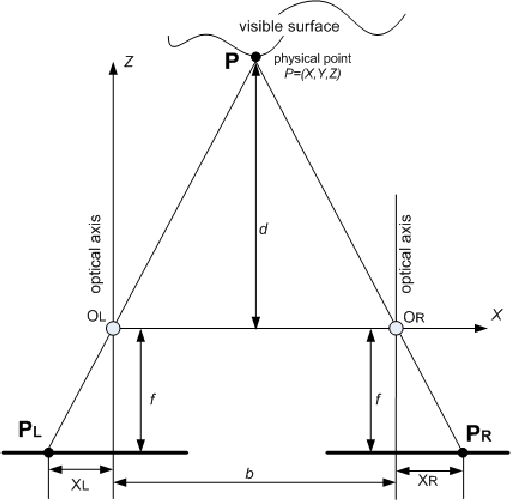
\includegraphics[height=0.5\textheight]{imgs/stereo.png}
		\end{center}
	\end{itemize}
	\end{frame}
	
	\begin{frame}
	\frametitle{Literature Review}
	\begin{itemize}
	
	\item \textit{Open DR} : 
	
	\end{itemize}
	\end{frame}
	
	\begin{frame}
	\frametitle{Literature Review}
	\begin{itemize}
	
	\item \textit{Occupancy Networks} :
	\end{itemize}
	\end{frame}
	
	\begin{frame}
	\frametitle{Literature Review}
	\begin{itemize}
	
	\item \textit{DIB-R Renderer} :
	
	
	
	\end{itemize}
	\end{frame}
	
	
	
	\section{Proposed Methodology}
	\begin{frame}
	\frametitle{Proposed Methodology}
	\begin{itemize}
		\item \textbf{Differentiable Rendering} \\ 
		\begin{itemize}
			\item \textbf{What is rendering ?} \\
			The process of converting a 3D scene into a 2D image is called rendering.
			\item Rendering Pipeline :\\
			in OpenGL and such APIs decompose the process of rendering 3D scenes into a set of sequential user-defined programs,reffered to as shaders. While there are many shader types, the three most important shaders that should be present are :
			\begin{itemize}
				\item Vertex Shader
				\item Rasterization Shader
				\item Fragment Shader

			\end{itemize}
		\item The Vertex shader and Fragment shaders are defined such that they are differentiable. whereas the Rasterization shader is not differentiable.
			
		\end{itemize}
	\end{itemize}
	\end{frame}	
	\begin{frame}
		\frametitle{Proposed Methodology}
		\begin{center}
			\begin{figure}
				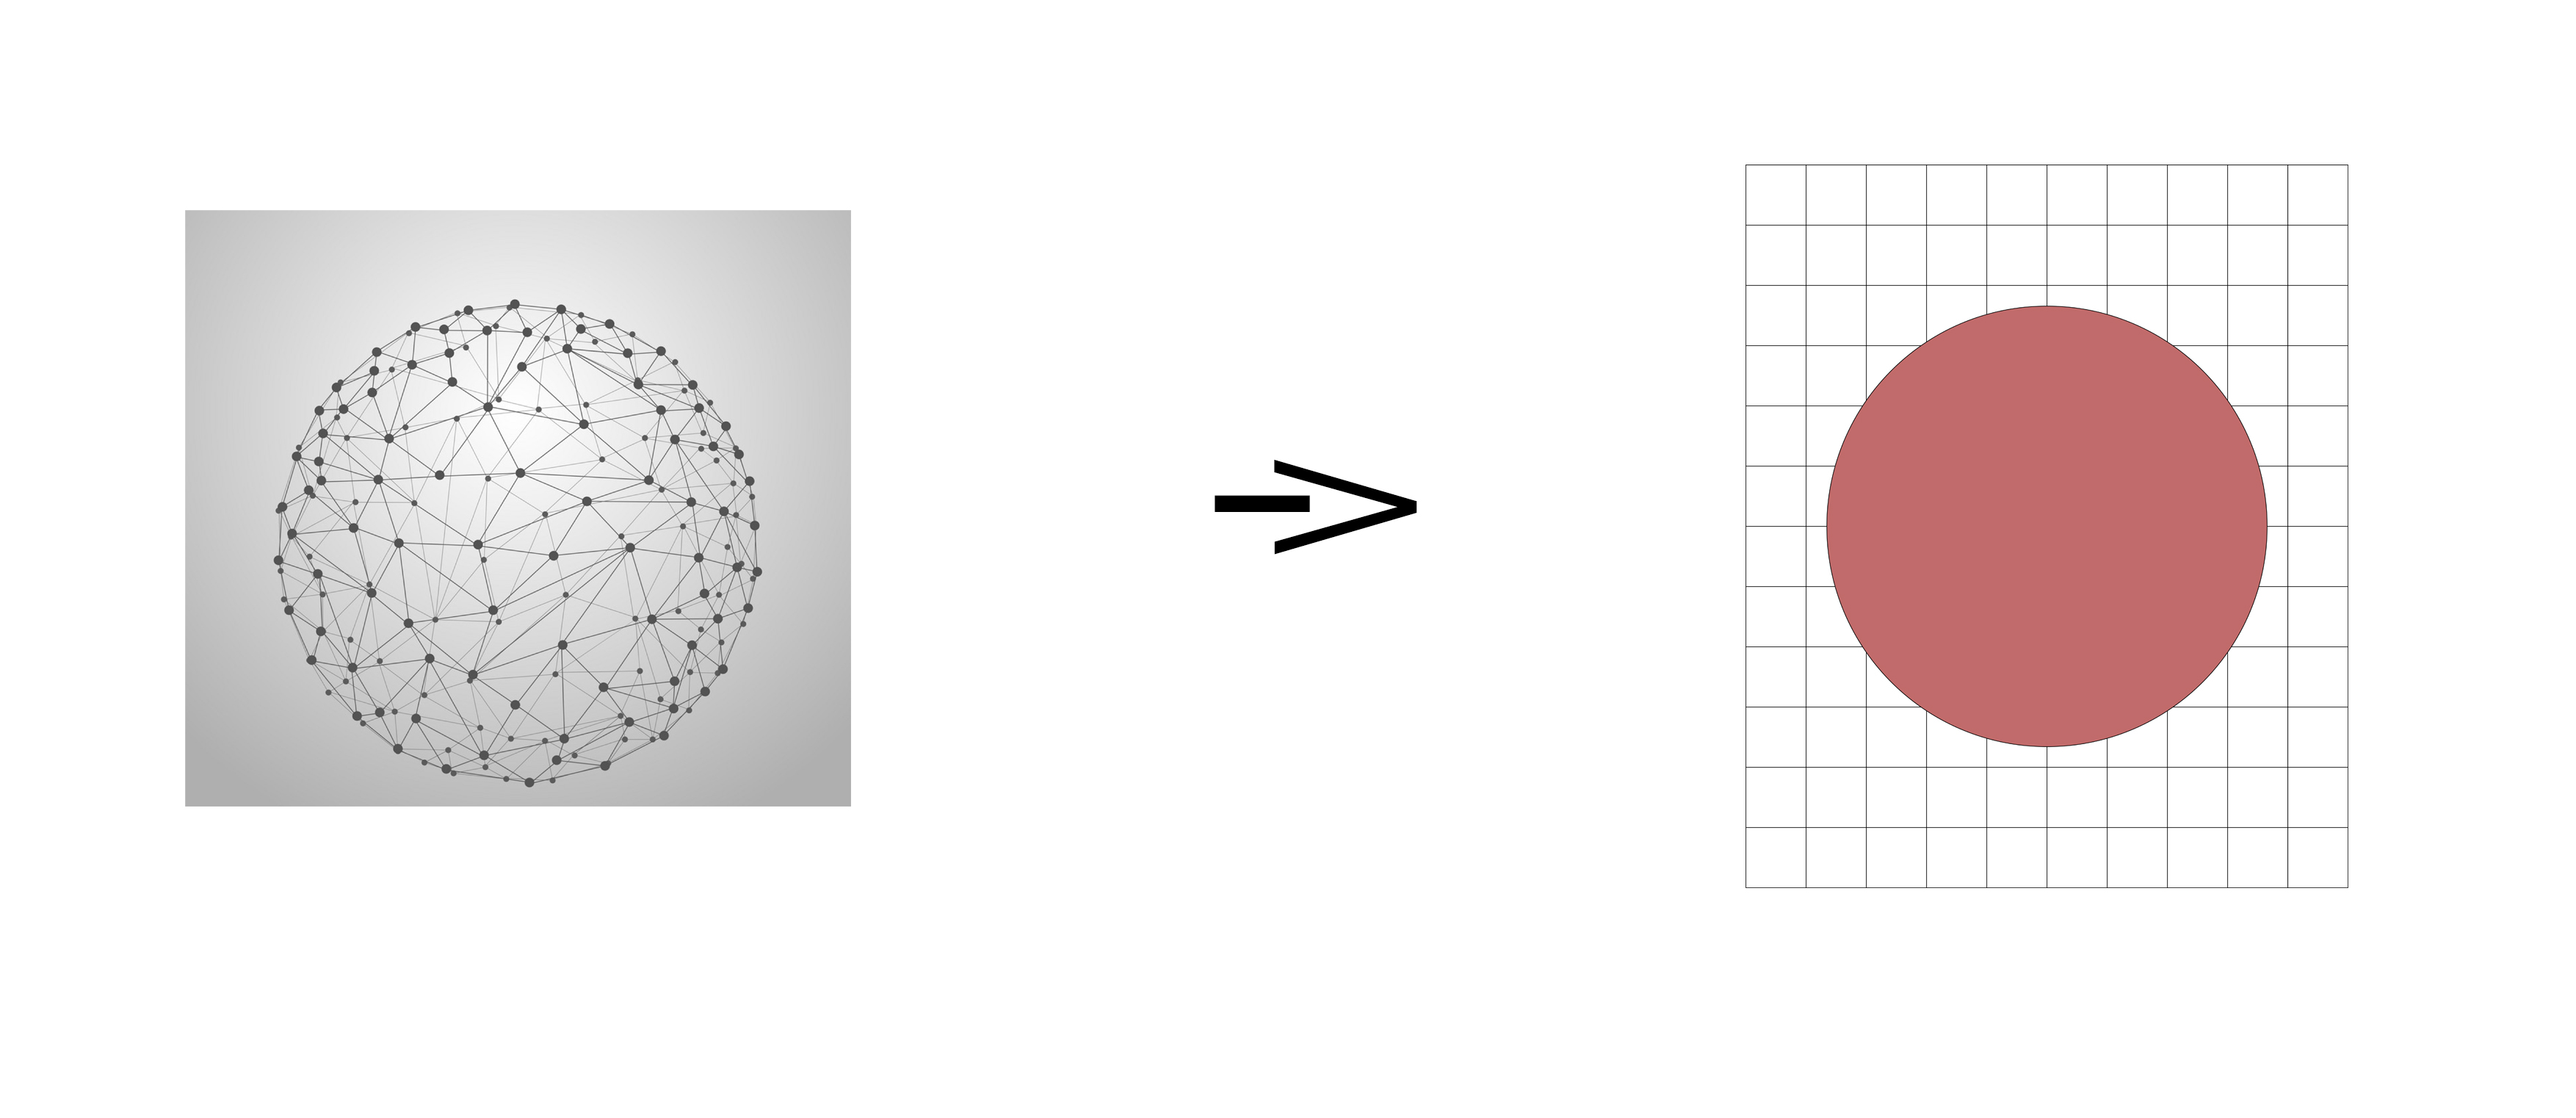
\includegraphics[height=0.3\textheight]{imgs/vertex.jpg}
				\caption{Vertex Shader}
			\end{figure}
			\begin{figure}
				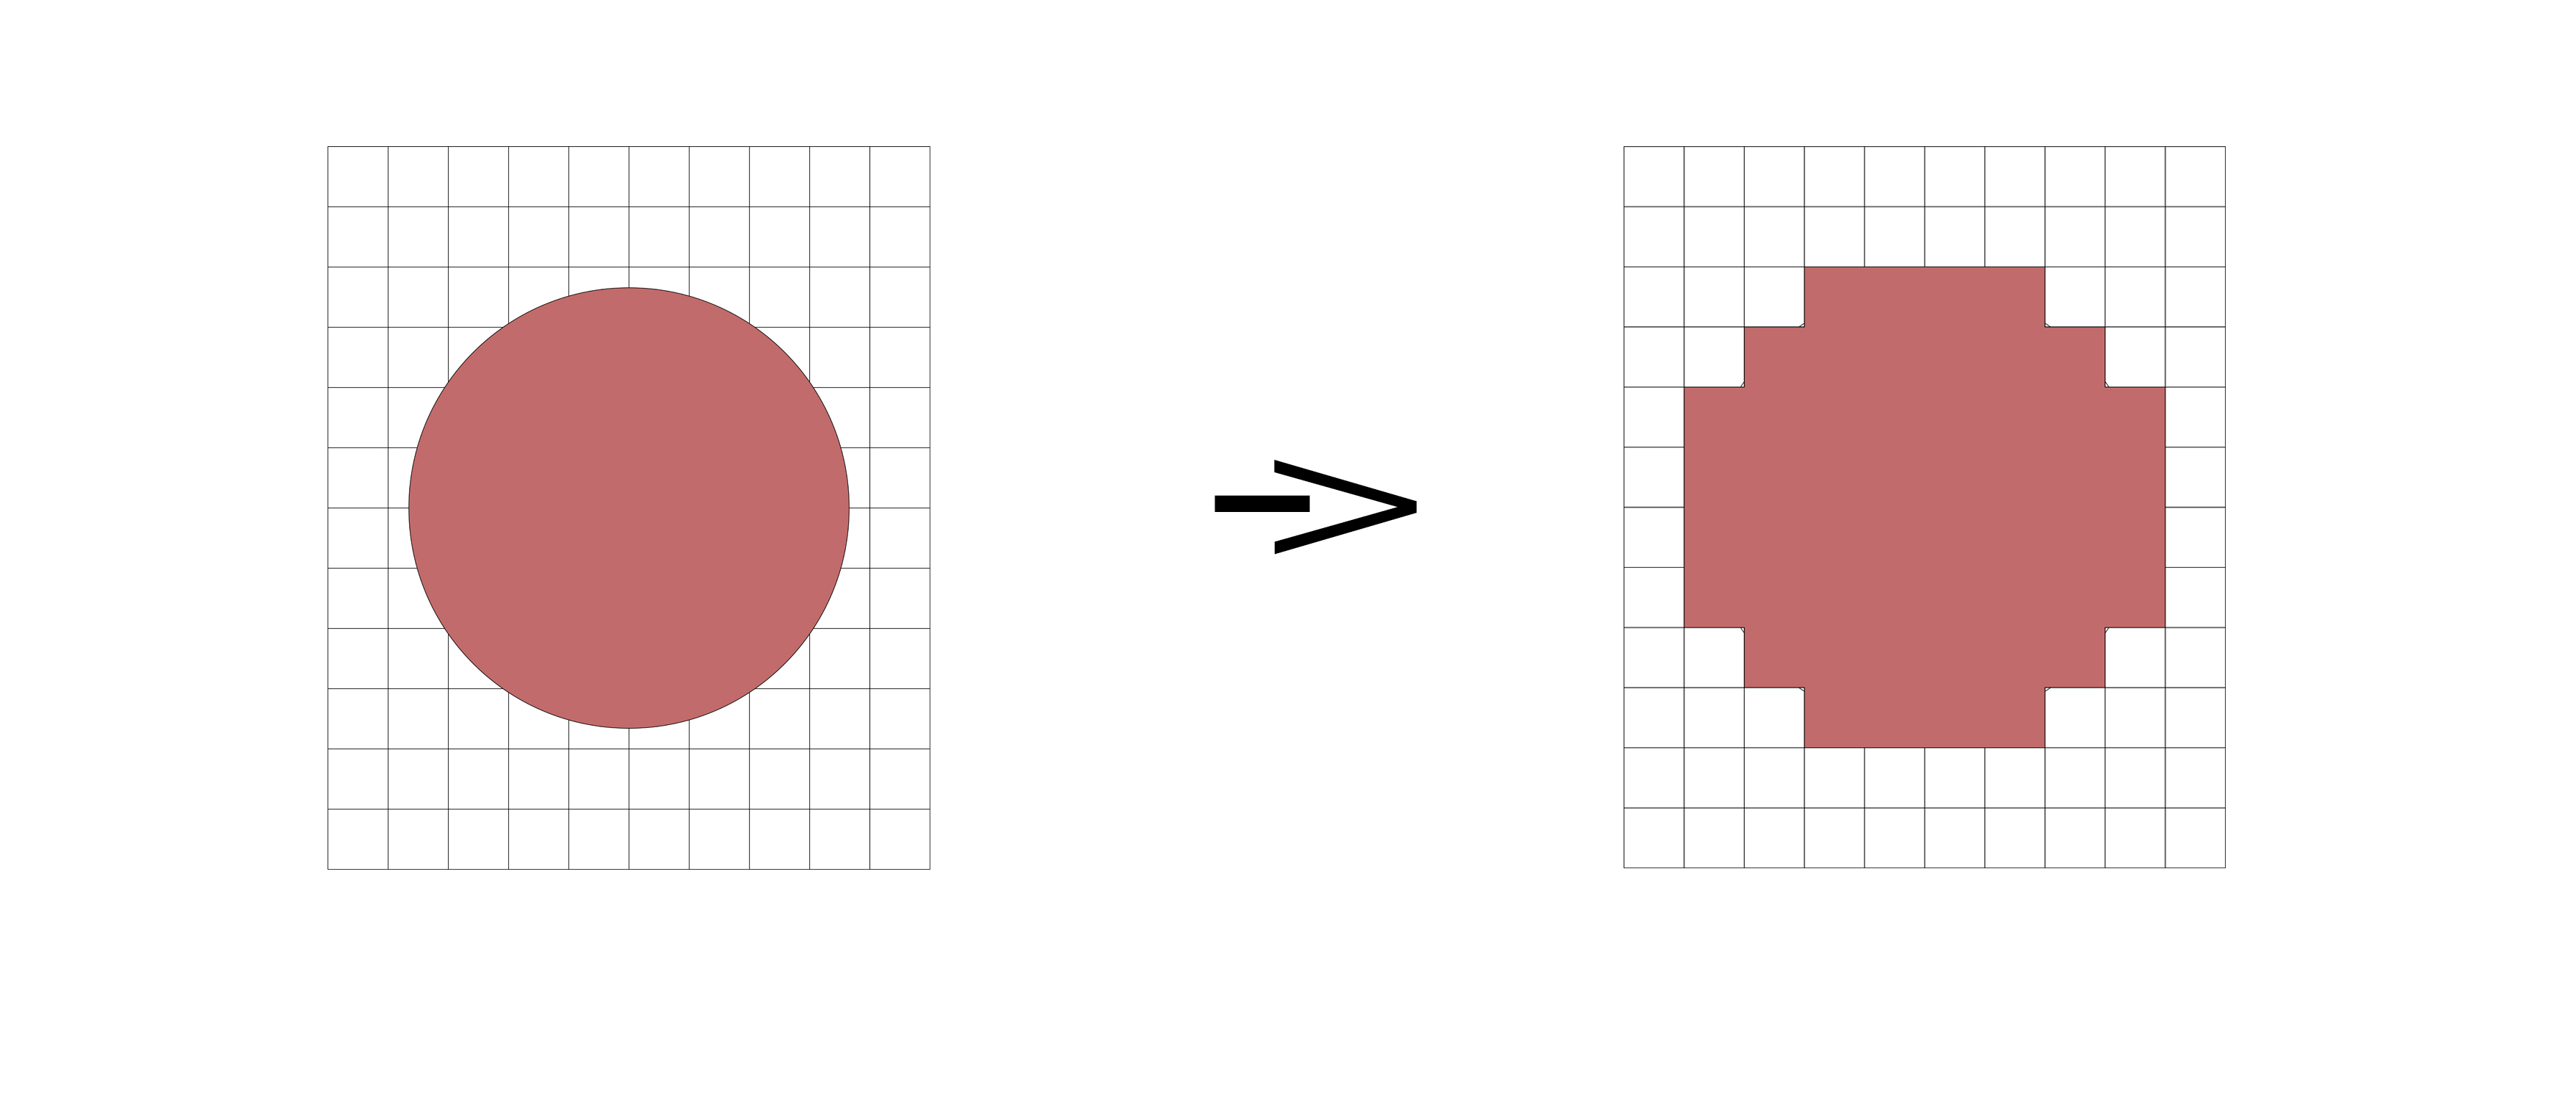
\includegraphics[height=0.3\textheight]{imgs/rasterization.jpg}
				\caption{Rasterization Shader}
			\end{figure}
		\end{center}
	\end{frame}
	\begin{frame}
		\frametitle{Proposed Methodology}
		\begin{columns}
			\column{0.5\textwidth}
			Using barycentric interpolation of the face's vertex attributes,
			
	%		\begin{block}{Formula}
    %			calculated in this equation
    %			\begin{equation}
    %       		Total = \frac{1}{n}*\sum_{i=0}^n (eachnode_i)
    %			\end{equation}
	%		\end{block}
	
			\begin{equation}
				I_{i} = u_{0}w_{0} + u_{1}w_{1} + u_{2}w_{2}
			\end{equation}
			\begin{equation}
				w_{k} = \Omega_{k} (v_{0} , v_{1} , v_{2} , p_{i})
			\end{equation}
			
			
			
			\column{0.5\textwidth}
			\begin{figure}
				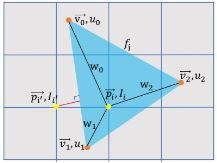
\includegraphics[width=0.8\textwidth]{imgs/dr.jpg}
				\caption{Illustration of differentiable renderer}
				
			\end{figure}
			
		\end{columns}
		
		The design of this differentiable renderer allows for optimization over all defined vertex attributes and a variety of rendering models, the L-1 loss between target images and predicted images is optimized.
	\end{frame}
	
	\begin{frame}
	\frametitle{Algorithm}
		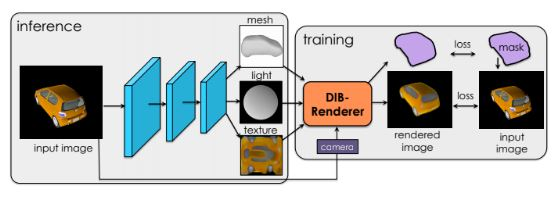
\includegraphics[width=\textwidth]{imgs/workflow.jpg}
	\end{frame}
	
	\section{Bibliography}
	\begin{frame}
		\frametitle{Bibliography}
		\printbibliography
	\end{frame}
	
\end{document}